\documentclass[main]{subfiles}
\begin{document}

%%@@@@@@@@@@@@@@@@@@@@@@@@@@@@@@
%\noindent
%\textbf{Topics: Interacting Neural Populations and Population Codes - 12.12.2019} \\
%Lecturer: Dr. Matthew Cook \\
%Author: Vanessa Leite \{vanessa at ini.uzh.ch\}

\section{Interacting Neural Populations}

\subsection{Neural Encoding of Information}

How the neurons encoding/process information?
We would like to understand it in a mechanistic level.
To understand the brain, we need to understand its structure and functionality (processes).
Different areas in the brain are highly connected, practically from any area you can reach, virtually, any other area.

Humans are capable to learn things that we were not evolved for, for instance, to fly a drone.
This is an inspiration for us.
It seems to exist a general solution for solving problems: the brain.

Neurons respond to \textbf{combinations} of properties, features, aspects of the situation, etc.
Neurons are tuned to a set of values for the parameters they care about.
For example, a neuron can be ``tuned" to a moving bar at a certain angle in its perceptive field. It also responds to a certain velocity, position (x,y), bar width, etc.

Neurons response is called firing rates. Although neurons are tuned, they aren't super picky about the exact values. And, experimentally, neurons do not code a single atributte but a combination of them.

\paragraph{Population code}

Information is encoded by a group (population) of neurons. A group includes all neurons in that area. The values are encoded by pattern of activity.

Given a parameter, and looking at the neurons tuned to some value of this parameter, we can define tunning curves.
In Figure~\ref{fig:tuning-curve}, we see in the $x$ axis the parameter we are evaluating, and in the $y$ axis, the activity of one single neuron (firing response).
Doing this process to many neurons, we can sort them regarding to the parameter we are looking for.
In Figure~\ref{fig:cell-order} all neurons were ordered accordingly to the response to a specific parameters.

The read out of information given a population code is an easy way to figure out what the population is doing, it is robust to noise, however, requires a lot of units.

\begin{figure}[H]
	\centering
	\begin{subfigure}[b]{0.3\textwidth}
		\centering
		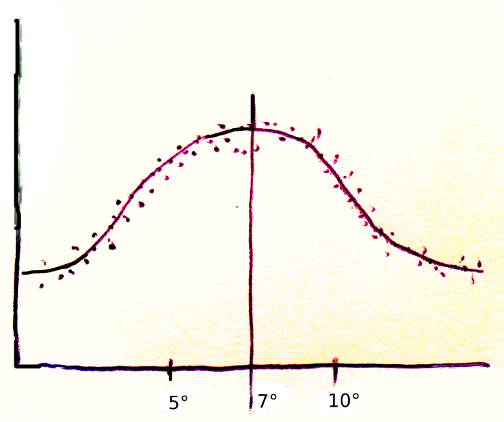
\includegraphics[width=\textwidth]{one-cell-tuning-curve.png}
		\caption{Tuning curve of one cell}
		\label{fig:tuning-curve}
	\end{subfigure}%
	~
	\begin{subfigure}[b]{0.3\textwidth}
		\centering
		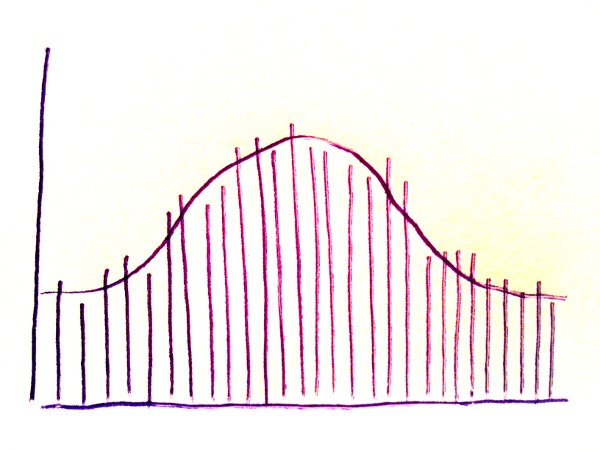
\includegraphics[width=\textwidth]{cell-order.png}
		\caption{Cells ordered by response to $20^\circ$}
		\label{fig:cell-order}
	\end{subfigure}
	~ 
	\begin{subfigure}[b]{0.3\textwidth}
		\centering
		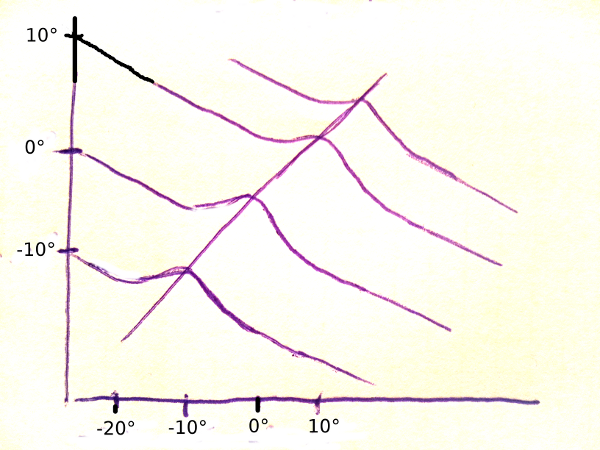
\includegraphics[width=\textwidth]{3D-visualisation.png}
		\caption{3D visualization of cell's response to different degrees}
		\label{fig:3d}
	\end{subfigure}
\end{figure}

Consider now an example were we want to correlate the angle of the eye (E), the position of an object on retina (R) and the head-centered direction (A), as showed in Figure~\ref{fig:APE}.
This is an example of processing that is not feed-forward.

How can a relation like $A = E + R$ be represented?
Say $R$, $A$ and $E$ are encoded by population codes, i.e., by population of units, each tuned to a particular value of that variable. Considering these three variables, we can use units that are tuned to combinations of A, E and R.
The set of $(A, E, R)$ triples that satisfy the relation will be active.
This can be seen in Figure~\ref{fig:REA}: when certain neuron fires for a parameter in $R$, another one can fire for a parameter in $E$ and this can result in the firing of neurons in $E$, after learning.
Given any two information in this relation, the third one can be recovered. There is no obligatory order.

$R$, $A$ and $E$ have the following relations:
\begin{itemize}
\item $R = A - E$
\item $A = E + R$
\item $E = A - R$
\end{itemize}

\begin{figure}[H]
	\centering
	\begin{subfigure}[b]{0.5\textwidth}
		\centering
		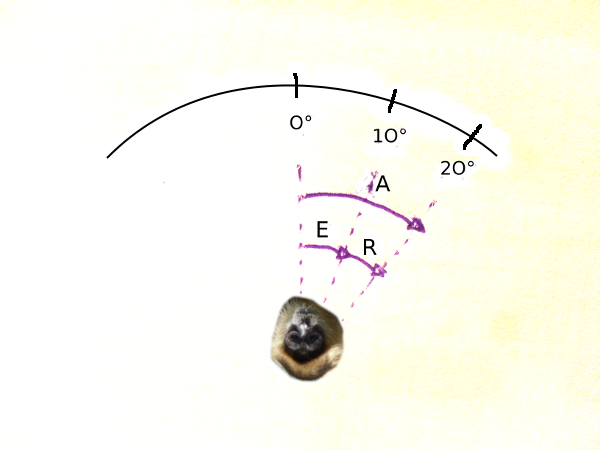
\includegraphics[width=\textwidth]{ape-picture.png}
		\caption{Monkey holding gaze fixed on point $10^\circ$ and light falling in from $20^\circ$}
		\label{fig:APE}
	\end{subfigure}%
	~
	\begin{subfigure}[b]{0.5\textwidth}
		\centering
		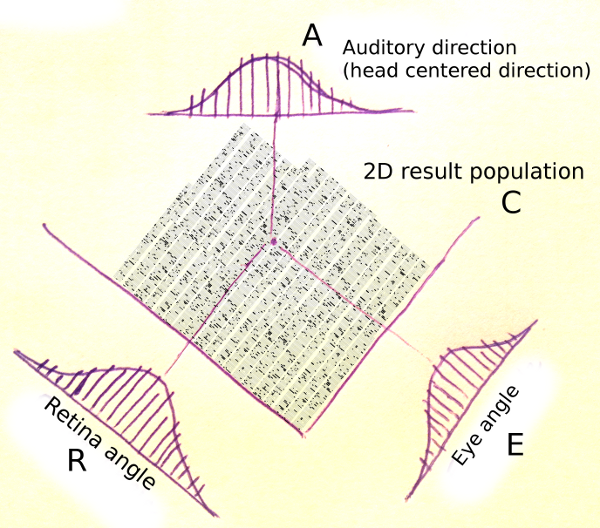
\includegraphics[width=\textwidth]{Retina-Eye-Auditory.png}
		\caption{Visualization of Retina angle ordering cell set R, Eye angle ordering set E,2D result population C and auditory direction set A.}
		\label{fig:REA}
	\end{subfigure}
\end{figure}

%\begin{figure}[H]
%	\centering
%	\begin{subfigure}[b]{0.3\textwidth}
%		\centering
%		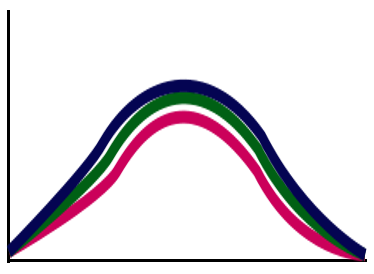
\includegraphics[width=\textwidth]{Cell-A.png}
%		\caption{Cell A $\in$ R}
%	\end{subfigure}%
%	~
%	\begin{subfigure}[b]{0.3\textwidth}
%		\centering
%		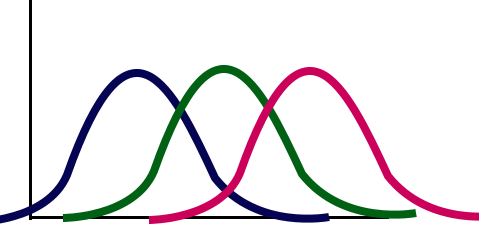
\includegraphics[width=\textwidth]{Cell-B.png}
%		\caption{Cell B $\in$ A}
%	\end{subfigure}
%	~ 
%	\begin{subfigure}[b]{0.3\textwidth}
%		\centering
%		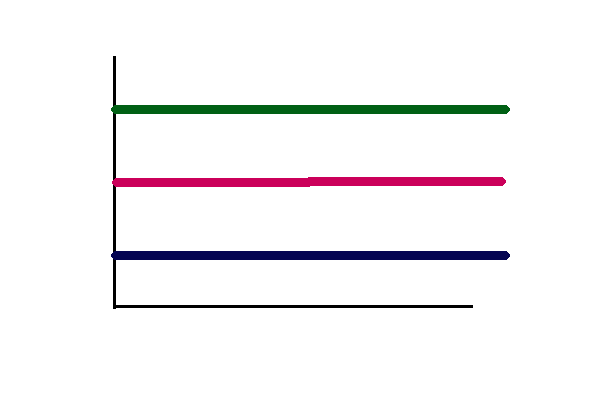
\includegraphics[width=\textwidth]{Cell-C.png}
%		\caption{Cell C $\in$ E}
%	\end{subfigure}
%\end{figure}
%
%\begin{figure}[H]
%	\centering
%	\begin{subfigure}[b]{0.3\textwidth}
%		\centering
%		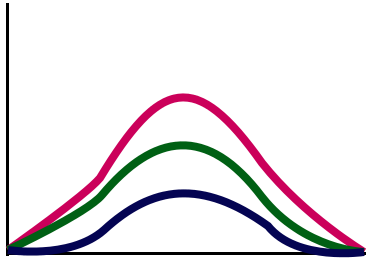
\includegraphics[width=\textwidth]{Cell-D.png}
%		\caption{Cell D $\in$ C}
%	\end{subfigure}%
%	~
%	\begin{subfigure}[b]{0.3\textwidth}
%		\centering
%		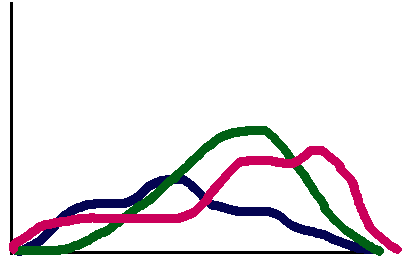
\includegraphics[width=\textwidth]{Cell-E.png}
%		\caption{Cell E (Not every neuron shows clear tuning curves)}
%	\end{subfigure}
%\end{figure}

\paragraph{Summary}
\begin{itemize}[noitemsep,nolistsep]
	\item Neurons can represent information through population codes.
	\item Neurons are tuned to preferred stimuli.
	\item Information is represented by the pattern of activity in a neural population.
	\item Each neuron has a preferred input, for example orientation, that it responds to. The neuron is tuned to that value.
	\item Not every neuron shows clear tuning curves.
	\item Neurons usually do not only respond to their preferred stimulus, but also with decaying strength to close ones.
	\item Population encoding has an easy read out value.
	\item Population encoding is robust to noise.
	\item Population encoding requires a lot of units.
\end{itemize}

\end{document}
